\documentclass[12pt]{article}

\usepackage[english]{babel}
\usepackage[utf8x]{inputenc}
\usepackage{pdfpages}
\usepackage{lastpage} % Required to determine the last page for the footer
\usepackage{extramarks} % Required for headers and footers
\usepackage{graphicx} % Required to insert images
\usepackage{listings} % Required for insertion of code
\usepackage{courier} % Required for the courier font
\usepackage{color}
\usepackage{grffile}
\usepackage{float}

% Margins
\topmargin=-0.45in
\evensidemargin=0in
\oddsidemargin=0in
\textwidth=6.5in
\textheight=9.0in
\headsep=0.25in
\fboxsep=0mm%padding thickness
\fboxrule=2pt%border thickness

\linespread{1.1} % Line spacing

\newcommand{\Title}{Software requirement specification} % Assignment title
\newcommand{\Class}{Cos\ 301} % Course/class
\newcommand{\pd}{Post-Doctoral}
\newcommand{\ssr}{Soft\color{green}{Serve }\color{black}}
\begin{document}

\vspace{4em}

\begin{center}%

\begin{figure}[ht!]
\centering

\includegraphics{./Pictures/logo.png}
\end{figure}
\LARGE \bf \Title \\
{\bf Version 0.5}\\[4em]
\LARGE {\bf \ssr Group }\\[1em]
\LARGE {\bf Members:}\\[2em]
\large
Kgothatso Phatedi Alfred Ngako (12236731) \\[1em]
Tokologo “Carlo” Machaba (12078027) \\[1em]
Mathys Ellis (12019837) \\[8em]

\end{center}%

%\newpage
%{\LARGE \bf Change log}\\[2em]

\begin{center}
\begin{tabular}{|l|p{1.4cm}|p{8cm}|p{2.8cm}|}
\hline
\multicolumn{4}{|c|}{\bf Change log} \\
\hline
 Date & Version & Description &  Person \\
\hline
10/02/2014 & v 0.0 & Document created & Mathys Ellis \\
\hline
02/03/2014 & v 0.1 & Added to glossary & Mathys Ellis \\
\hline
04/03/2014 & v 0.2 & Added Integration requirements, Architecture constraints, Functional requirements introduction & Alfred Ngako \\
\hline
05/03/2014 & v 0.3 & Added Introduction, Vision, Background, Access Channel requirements & Carlo Machaba \\
\hline
06/03/2014 & v 0.4 & Added domain objects, open issues. Modified some sections & Alfred Ngako \\
\hline
06/03/2014 & v 0.5 & Added quality requirements, methodology, scope and limitations & Mathys Ellis \\
\hline
08/03/2014 & v 0.6 & Added some wrapping to the change log which is now a table & Alfred Ngako \\
\hline
11/03/2014 & v 0.7 & Added more functional requirements which relate more to the use case diagrams & Alfred Ngako \\
\hline
16/03/2014 & v 0.8 & Added domain objects data relation diagrams & Alfred Ngako \\
\hline
16/03/2014 & v 0.8 & Added some preconditions and did some formatting & Mathys Ellis \\
\hline
17/03/2014 & v 0.8 & Added rest of preconditions and all the postconditions. Also added to the glossary & Mathys Ellis \\
\hline
20/03/2014 & v 0.9 & Updated the domain objects diagram  & Mathys Ellis \\
\hline
20/03/2014 & v 0.9 & Updated the domain objects plus diagram  & Alfred Ngako \\
\hline
\hline
20/03/2014 & v 0.9 & Updated the use case prioritizaion  & Alfred Ngako \\
\hline

%\end{tabbing}
\end{tabular}
\end{center}
\newpage
\tableofcontents

\listoffigures
\newpage
\section{Introduction} %Carlo
A Post-Doctoral fellow is a person who conducts research after they have completed their PhD, with the aim of deepening their knowledge in a specific field. The University of Pretoria supports such research opportunities in order to the increase research output of the University. Post-Doctoral fellows who conduct their research at the University of Pretoria do so under the supervision of a staff member of the University and their research may be privately or internally funded. This is a growing field in Universities around South Africa. Thus a lack in the IT services for the application management of Post-Doctoral fellow has been spotted by SoftServe.
\vspace{0.2in}

\subsection{Purpose:}
\vspace{0.2in}
This Software Specifications Requirements document serves the purpose of providing a detailed overview of the non-functional and functional requirements as well the goals that SoftServe's Post-Doctoral application management system wishes to satisfy. Further it defines the abstract interaction of stakeholders with the system. Thus this document serves as a contract between SoftServe and the client, Mrs Cathy Sandis of the DRIS of the University of Pretoria.

\vspace{0.2in}

\subsection{Document Conventions:}
\vspace{0.1in}
\begin{itemize}
\item Documentation formulation: LaTeX
\item ERD Crow-Foot notation
\item UML 2.0
\end{itemize}

\vspace{0.2in}

\subsection{Project Scope:}
\vspace{0.2in}	
The scope of the project is to design a Post-Doctoral application management system where prospective or current Post-Doctoral fellows can apply for or renew fellowships at the University of Pretoria. The system will then further allow the management of such applications/renewals till the end of the application process. The end is defined as: DIRS have approved the application and have notified the CSC and Finance department. The system will replace the current paper based system currently in place. The system will be designed so to allow for future integration with the current student and personnel management system, PeopleSoft, employed by the University of Pretoria. Though the scope of this SRS document will be to make the system and have it independent of any other system.
\vspace{0.2in}

\subsection{References:}
\vspace{0.1in}
\begin{itemize}
\item Dr.Phol, K., 2010, \textit{Requirements Engineering: Fundamentals, Principles, and Techniques}, Springer, Heidelberg.
\end{itemize}	

\vspace{0.5in}

\section{Vision} %Carlo
\vspace{0.2in}
The client needs a system which can make the management of the application and renewal processes of Post-Doctoral fellowships more effective, reliable, secure and audit-able. Together the client and SoftServe have envisioned a system that will make use of a centralised user friendly web interface that will be used by the prospective fellows and all the stakeholders involved in the application and renewal processes. The system will have various sections that handle the different stages in the process. The system will need to automate the transitions between phases by forwarding the required information to the next stakeholder in the process and notifying them via a email notification. The system will also need to provide reporting facilities for the information stored by the system. As well as progress tracking with regards to any application or renewal. The system data needs to be centralised to ensure that any information used by system is cohesive and valid for any stakeholder who accesses it. By introducing a digital system that is not paper based, the client hopes that the application and renewal processes will be easier to track and manage.
\vspace{0.5in}

\section{Background} %Carlo
\vspace{0.2in}
The current Post-Doctoral application and renewal processes are paper based thus there are a number of drawbacks, mainly due to human error. One such drawback is that there is no audit trail when it comes to the different stakeholders input involved in approving or declining the applications. Another involves the minutes of Post-Doctoral committee meetings which are often misplaced or typed in an inconsistent manner making it hard to recall what has been discussed in the meetings that evaluate prospective applications and renewals. Access to documents is also a problem since they are usually hard copies that change hands constantly thus the process of getting hold of the documents is long and often tedious if not made impossible if they are lost. Reporting on the information of fellows, renewals and even communication with already approved fellows is also problematic, because the current system is not centralised. Therefore gathering all the information required to generate the reports is difficult or even impossible. This is where the client Mrs Cathy Sandis saw a potential area that could be optimised by the implementation of digitalised system. This is where the SoftServe group was brought into the picture.
\vspace{0.5in}

\newpage
\section{Methodology} %Mathys
\vspace{0.2in}

This document was created using the requirement elicitation techniques and requirement definitions specified in Klaus Pohl’s book Requirements Engineering: Fundamentals, Principles, and Techniques [Dr.Phol, K., 2010].
The requirements were elicited from the following sources:
\begin{itemize}
\item Numerous interviews with the client
\item Collecting and analysing various documents such as:
\begin{itemize}
\item The initial project request document
\item Application forms
\item Renewal forms
\item CV templates
\item Approval and recommendation forms
\end{itemize}	
\item Online research into UP Post doctoral applications
\item Correspondence with the UP IT department
\end{itemize}	

\vspace{0.5in}


\newpage
\section{Stakeholders} %Mathys
\vspace{0.2in}

The stakeholders that will engage or be engaged by the system are listed below:

There are three categories under which stockholders can fall:
\begin{itemize}	
\item External:
These are stakeholders that do not have a PeopleSoft account or are fellows.
\begin{itemize}	
\item \textbf{Prospective fellow} - A person who wishes to renew or apply for a research position/fellowship.
\item \textbf{Referee} - A person who is identified by a Prospective fellow as a referral.
\end{itemize}

\item Internal individuals:
These are stakeholders that do have a PeopleSoft account and are individual members of staff.
\begin{itemize}	
\item \textbf{Grant holder} - The person who is a fellow's supervisor and a member of staff at the University of Pretoria. This is person is known also the applicant.
\item \textbf{HOD} - The head of the department of which a Grant holder is a member.
\end{itemize}
\item Internal groups:
These are stakeholders that do have a PeopleSoft account and are a group of staff members.
\begin{itemize}	
\item \textbf{Dean's office} - The dean and deputy dean of the faculty under which the department which the Grant Holder is a member of.
\item \textbf{DRIS} - The department of Research and Innovation Support at the University of Pretoria. This stakeholder oversees the application and renewal processes.
\item \textbf{Post-doctoral committee} - The committee who evaluates any post-doctoral fellowship applications and renewals.
\item \textbf{CSC} - The client service centre of the University of Pretoria.
\item \textbf{Finance} - The department of finance at the University of Pretoria.
\end{itemize}
\end{itemize}
\vspace{0.5in}

\newpage
\section{Architecture requirements}
\subsection{Access channel requirements} %Carlo
\vspace{0.2in}
All stakeholders: Will access the system through a HTML 5 web browser client that is locally installed on a user's computer system or mobile platform. Support for HTML 4.0.1 will also be implemented. The web interface will allow different stakeholders access to different sections of the system based on the roles assigned to their accounts.

\vspace{0.2in}

\subsection{Quality requirements} %Mathys
\vspace{0.2in}

\subsubsection{Availability:}

\begin{flushleft}

The system's availability on designated networks will depend on the availability of the University of Pretoria's servers that host the system. If the University of Pretoria's servers hosting the system are active and provide access over a designated network then the system must be available over that designated network. The designated networks are defined as the internet and the campus network of the University of Pretoria.

\end{flushleft}

\vspace{0.1in}

\subsubsection{Security requirements}

\begin{flushleft}

The system will need to be fully secured since the system deals with confidential information such as person information, application statuses, financial data and meeting information. Also since the systems main goal is to provide stable and audible application and renewal process flow the system may not be vulnerable to data tampering or any tampering whatsoever. \\
\vspace{0.1in}

The system will have to provide different security roles to the registered users on the system. Any number of roles should be assignable to any user by a administrator with the correct role to allow for flexibility.
But in essence a stakeholder may only have access to their section of the application process. The system administrator should be able to view all the sections in the system and should be able to modify them except where they may not.

\end{flushleft}

\vspace{0.1in}

\subsubsection{Scalability requirements}

\begin{flushleft}

The current aim is to create a scalable system that can support 500 to 1000 applicants per year with possible growth. This is in line with the figures given by the client and the growth in the research sector of the university.\\
\vspace{0.05in}

The system needs to be scalable in regard to the following factors:
\begin{itemize}


\item\textbf{Performance:} This is regarded as the speed and responsiveness of the system.
The system needs to be handle report queries in less than 10 seconds. It should be able to handle any application section processing in less than 3 seconds.\\

\item\textbf{Storage:} This is regarded as the growth and shrinking of the data that is stored.
The system will need to be able to handle a database that is in the range of 1 GB to 15 GB that has the potential to grow even larger. The reason for this stems from the requirement that the system will support archival functionality and archived data will store the data for long periods of time.\\

\item\textbf{Concurrency:} This regarded as the amount of active users on the system at the same time.
The system will need to support at least 100+/- concurrent users efficient and effectively since the system requires multiple stakeholders to part take in the application process while there can be multiple applications occurring at the same time.\\

\end{itemize}
\end{flushleft}
\vspace{0.1in}

\subsubsection{Testability:}

\begin{flushleft}

The system must be testable. This will be done using unit testing and following the test plan that will be laid out in the testing document of this project.\\

\vspace{0.1in}

Unit testing will test each unit in regard to:
\begin{itemize}

\item\textbf{Preconditions}
\item\textbf{Post conditions}

\end{itemize}

The project will also have two phases of testing:

\begin{itemize}

\item\textbf{Offline:} This is the initial phase of testing and debugging which will be done with pseudo data.
\item\textbf{Online:} This is the final phase of testing and debugging which will be done with active real time data.

\end{itemize}

\end{flushleft}

\vspace{0.1in}

\subsubsection{Auditability:}

\begin{flushleft}

The system needs to provide an audit trail of all critical actions that occur in the system. Critical actions are considered: user account management operations, login action, logout action and any operation by a user that leads to a change in application data of a particular prospective fellow.\\

\vspace{0.1in}

The Audit trail will be in the form of a read-only table stored in the database. It can only be viewed by a user with the correct security role. The system is the only entity that can modify the audit trail where this modification can only be the addition of entries.

\end{flushleft}
\vspace{0.1in}	

\subsubsection{Usability requirements}

\begin{flushleft}

The primary language of the system will be South African English. Any other language support is not considered part of the requirements but the system will be designed to allow for such development in the future.\\

\vspace{0.1in}

The system's UI will only consider 2 types of user categories with regard to usability:

\begin{itemize}

\item\textbf{Trained user:}

This type of user will have to have training in understanding how the system functions and how to use it. Their computer skills will be assumed to be in the range of basic to intermediate. Thus the user interface can allow for certain complexities but these complexities must be kept at a minimal. This user will be regarded as a system administrator. The stakeholders who fall under this category is the DRIS staff members overseeing the application process.

\item\textbf{Normal user:}

This type of user will have no training. Their computer skills will be assumed to be none or minimal. Therefore the UI that they will have access to will be simplistic and will be as user friendly as possible. The stakeholders that fall under this category will be Prospective fellows, Grant holders, HODs, Deans and Post-doctoral committee members.

\end{itemize}

\end{flushleft}

\vspace{0.2in}	


\subsection{Integration requirements} %Alfred
\vspace{0.2in}
The system has to integrate with the following systems:
\begin{itemize}
\item Must be able to create exportable data packages containing the information of approved fellowships that can easily be loaded into the CSC PeopleSoft system.
\item Must be able to query CSC PeopleSoft system to retrieve the account information of internal individuals/group Stakeholders to create a uniform login experience.
\item Must assign Prospective fellows with a id number in such a way that is integrable with UP Emplid. SoftServe suggests: "f" + 8 digit code.
\item Must be able to access and utilize the NRF researcher ratings.
\end{itemize}
\vspace{0.2in}

\subsection{Architecture constraints} %Alfred
\vspace{0.2in}
The following architecture constraints have been selected as being suitable for the system.
\begin{enumerate}
\item Database technology: MySQL
\item Development technology: Java EE
\item Web server: Apache Tomcat
\item Application server: GlassFish
\item Web interface protocol: HTTPS
\end{enumerate}
\vspace{0.5in}


\section{Functional requirements}
\subsection{Introduction} %Alfred
\vspace{0.2in}
This section discusses the functional requirements for the University of Pretoria's Post-Doctoral application management system. Highlighting the scope and limitations that are faced by the system. \linebreak \linebreak
The required functionality, domain objects and use cases related to the functional requirement will be discussed.
\vspace{0.2in}

\subsection{Scope and Limitations/Exclusions} %Mathys
\vspace{0.2in}


\subsubsection{Scope}
\vspace{0.2in}

\begin{figure}[H]
\centering	
\framebox{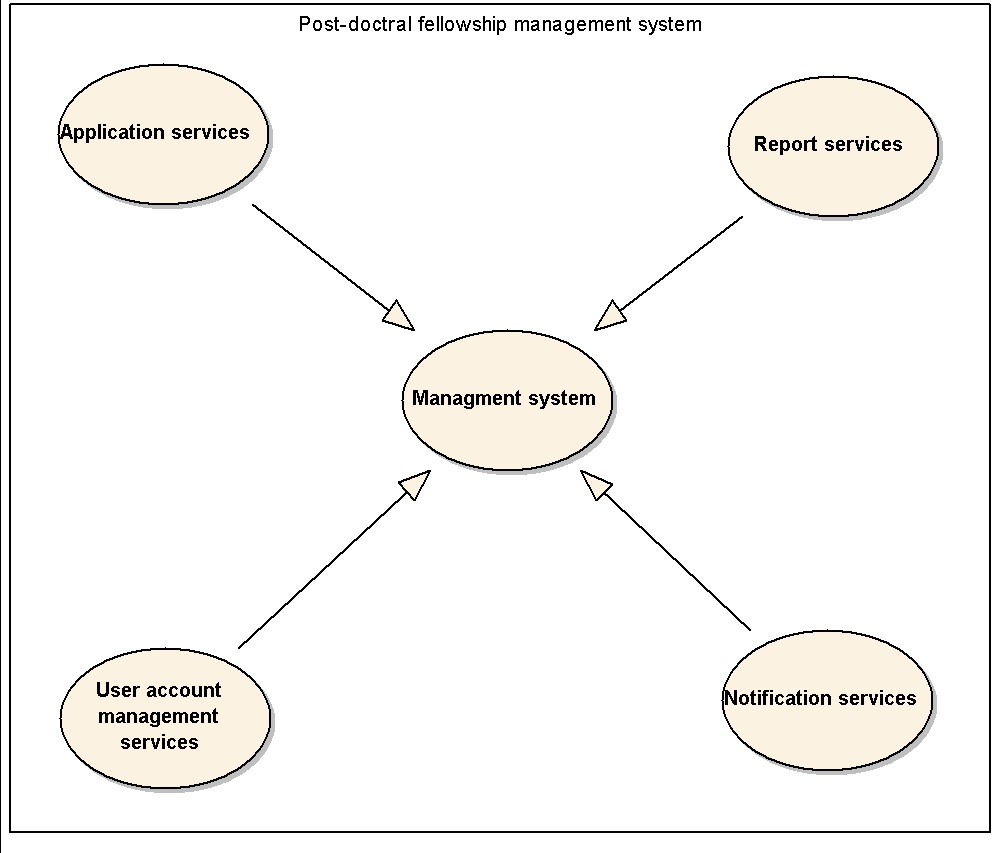
\includegraphics[scale=0.6]{./Pictures/Diagrams/Post-doctral fellowship management system.jpg}}
\caption{Use case diagram of Post-doctoral fellowship management system}
\end{figure}

\begin{figure}[H]
\centering	
\framebox{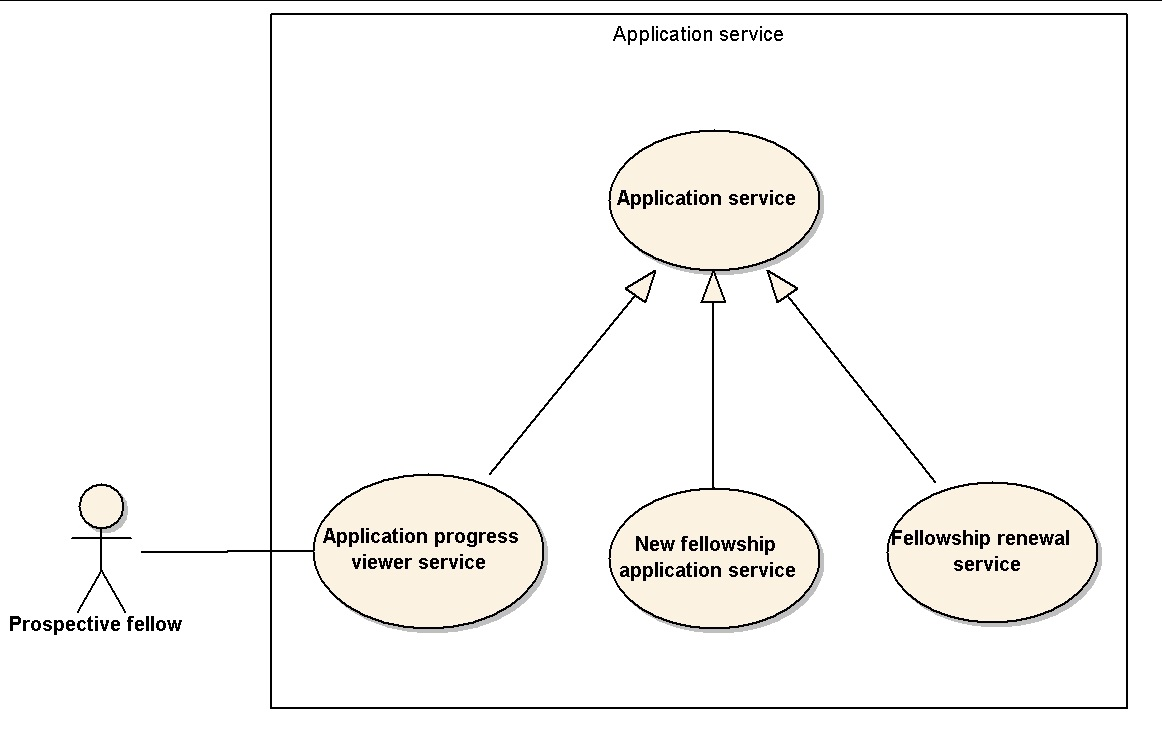
\includegraphics[scale=0.6]{./Pictures/Diagrams/Application service.jpg}}
\caption{Use case diagram of Application service}
\end{figure}

\begin{figure}[H]
\centering	
\framebox{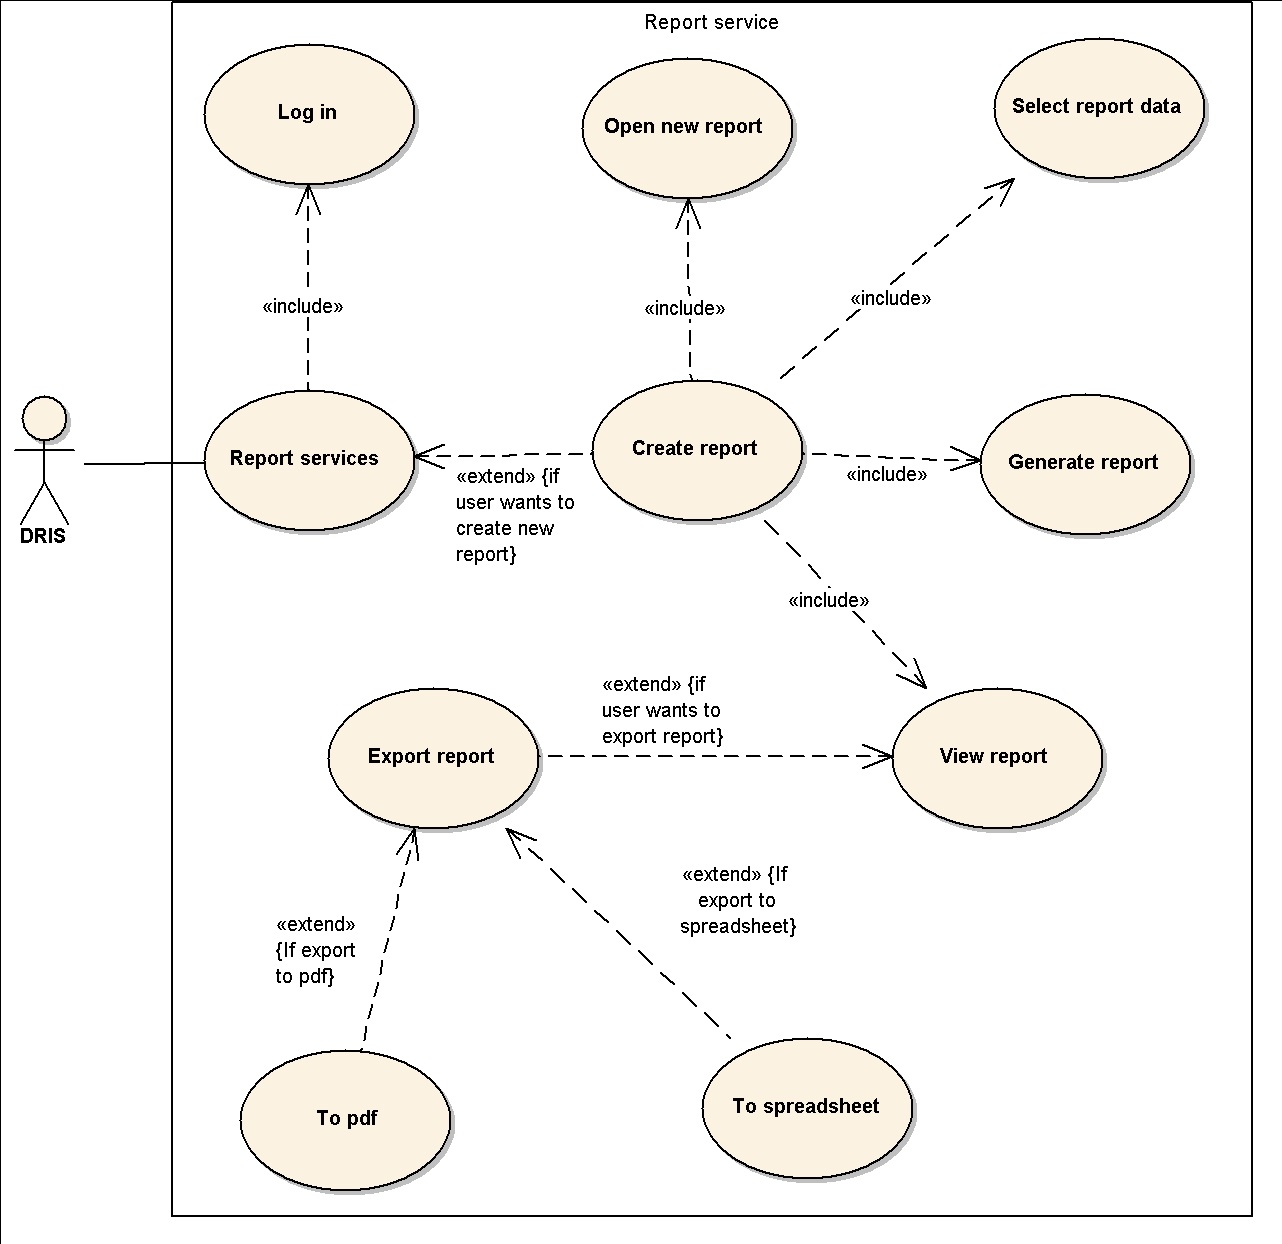
\includegraphics[scale=0.6]{./Pictures/Diagrams/Report service.jpg}}
\caption{Use case diagram of Report service}
\end{figure}

\begin{figure}[H]
\centering	
\framebox{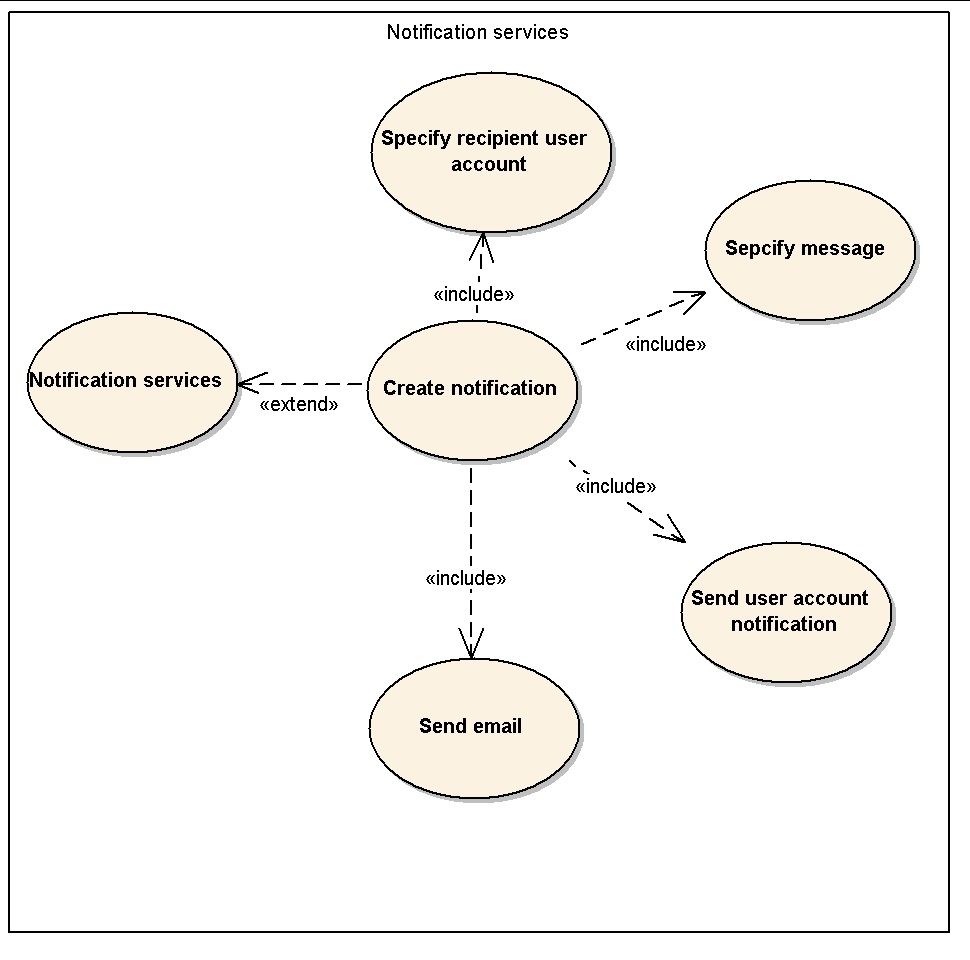
\includegraphics[scale=0.6]{./Pictures/Diagrams/Notification services.jpg}}
\caption{Use case diagram of Notification services}
\end{figure}

\begin{figure}[H]
\centering	
\framebox{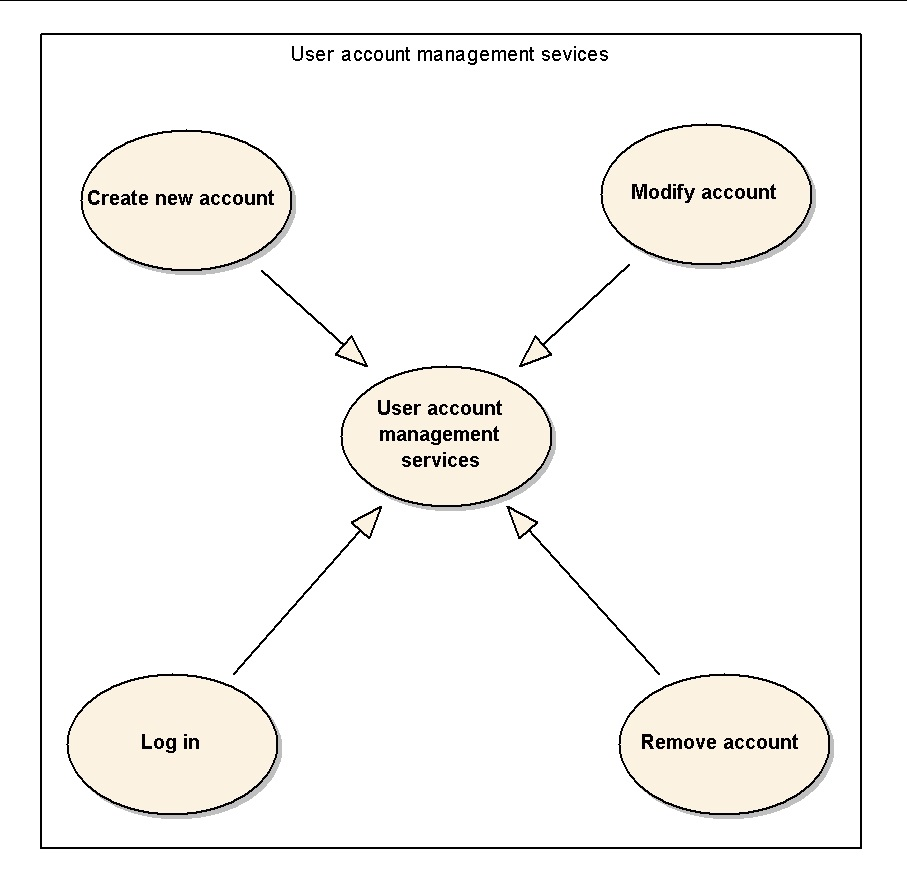
\includegraphics[scale=0.6]{./Pictures/Diagrams/User account management services.jpg}}
\caption{Use case diagram of User account management services}
\end{figure}

\begin{figure}[H]
\centering	
\framebox{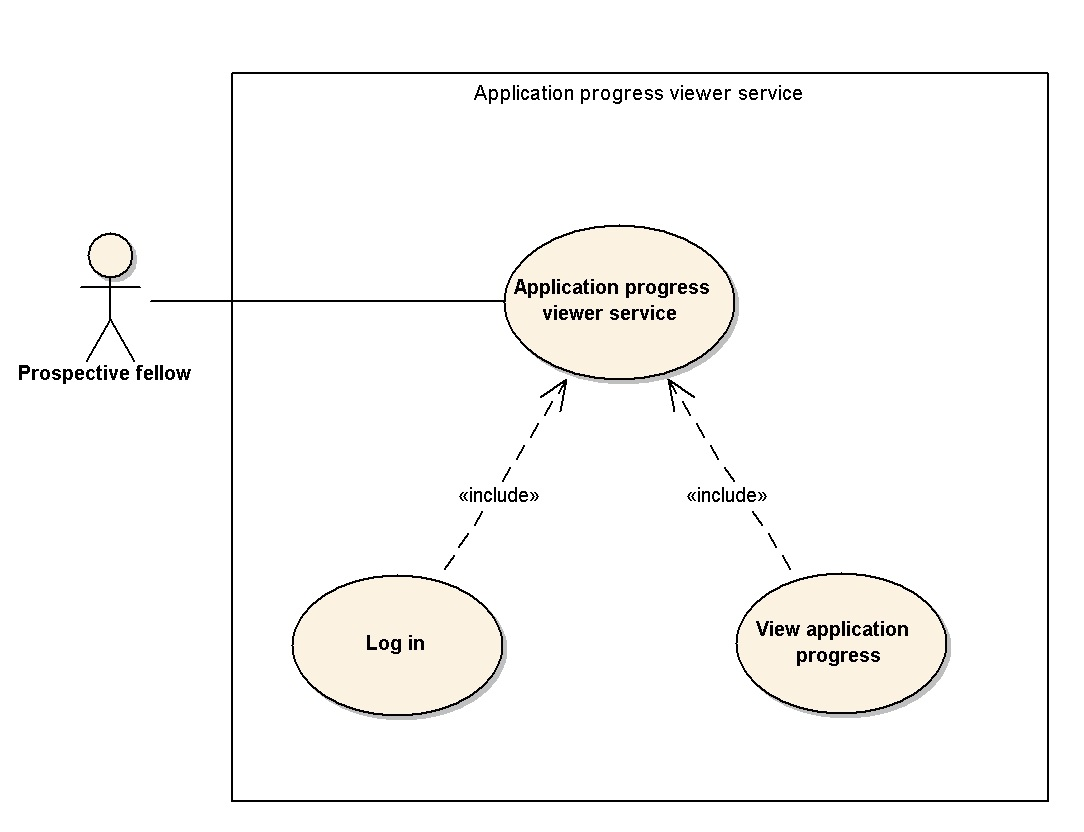
\includegraphics[scale=0.6]{./Pictures/Diagrams/Application/Application progress viewer service.jpg}}
\caption{Use case diagram of Application progress viewer service}
\end{figure}

\begin{figure}[H]
\centering	
\framebox{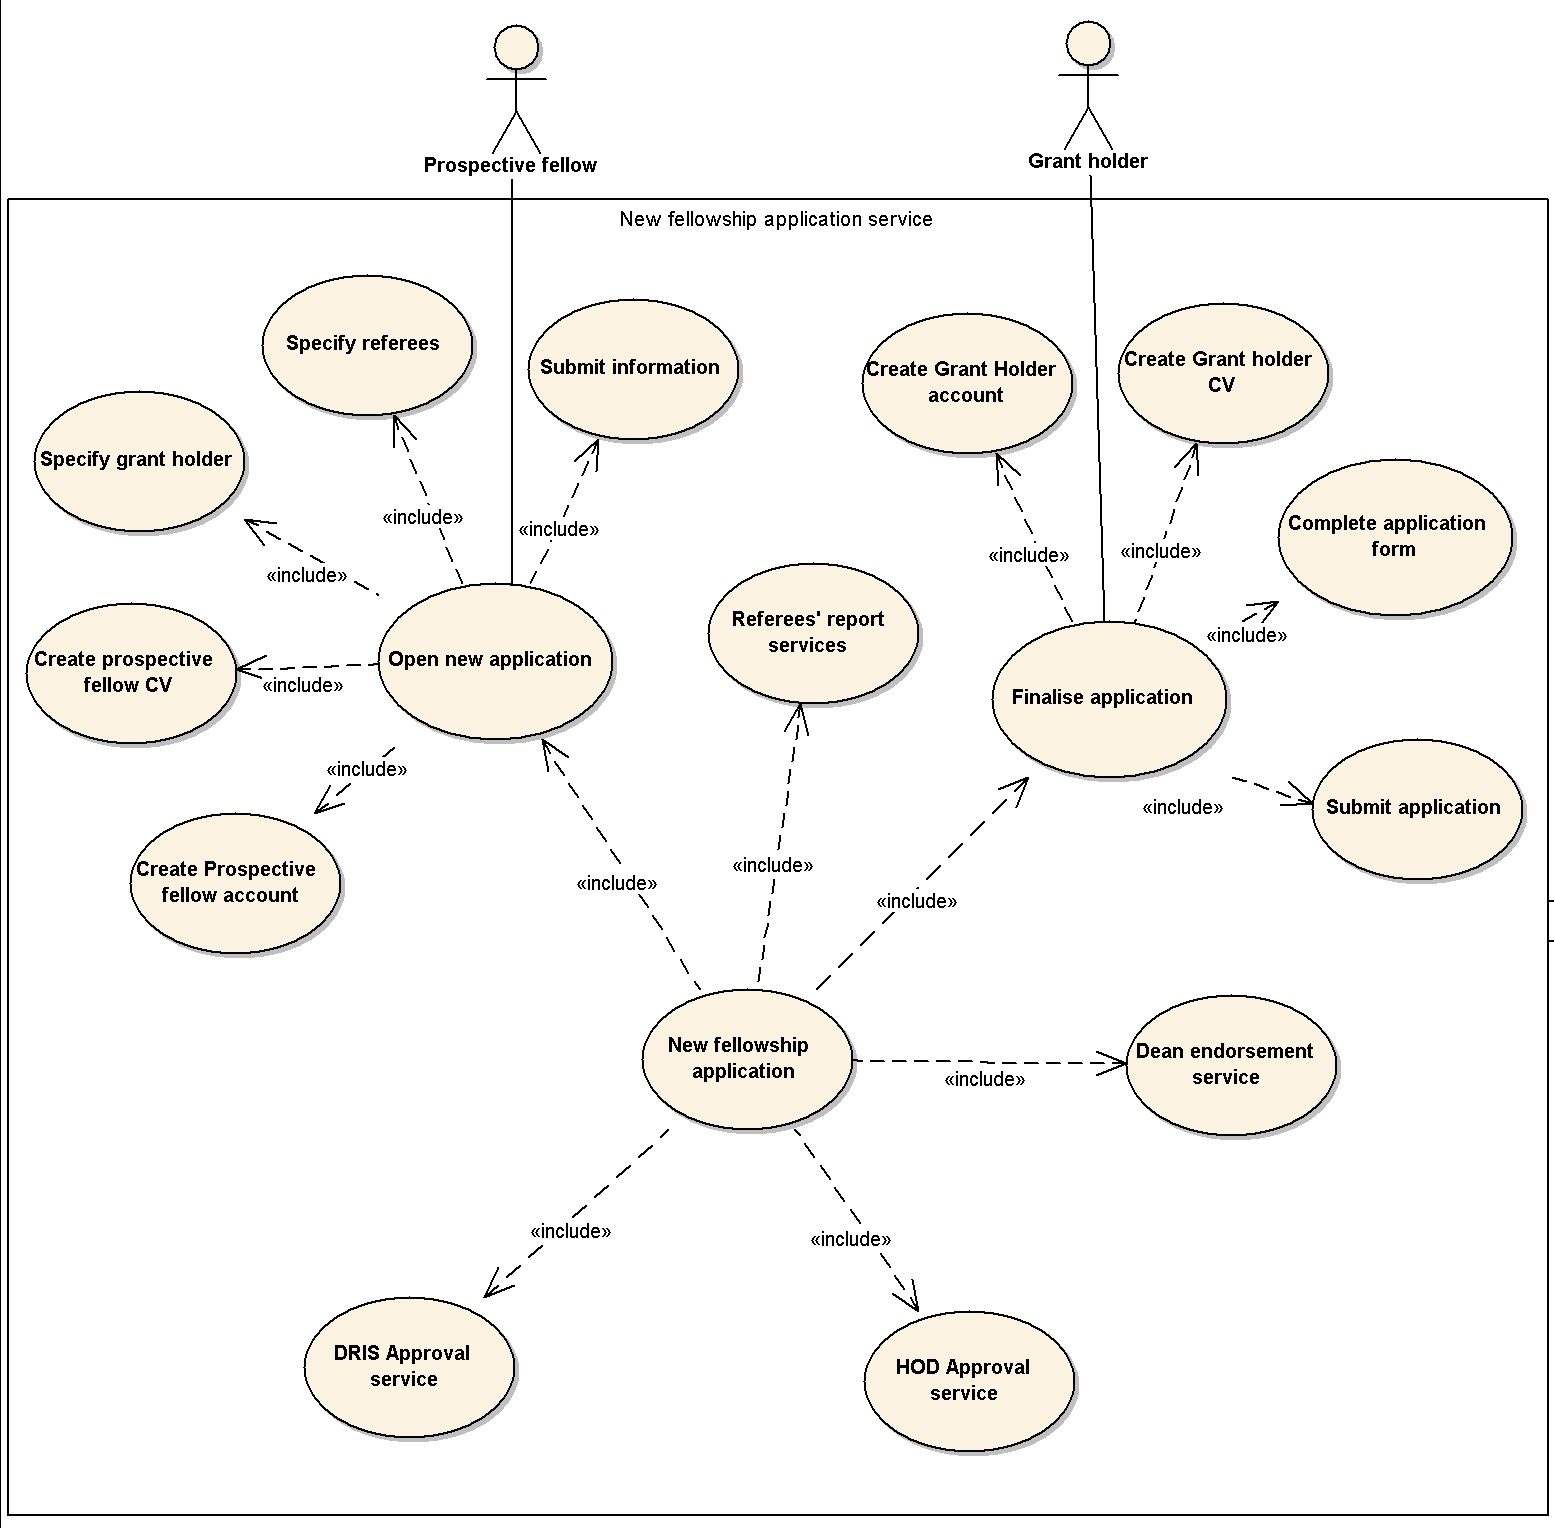
\includegraphics[scale=0.6]{./Pictures/Diagrams/Application/New fellowship application service.jpg}}
\caption{Use case diagram of New fellowship application service}
\end{figure}

\begin{figure}[H]
\centering	
\framebox{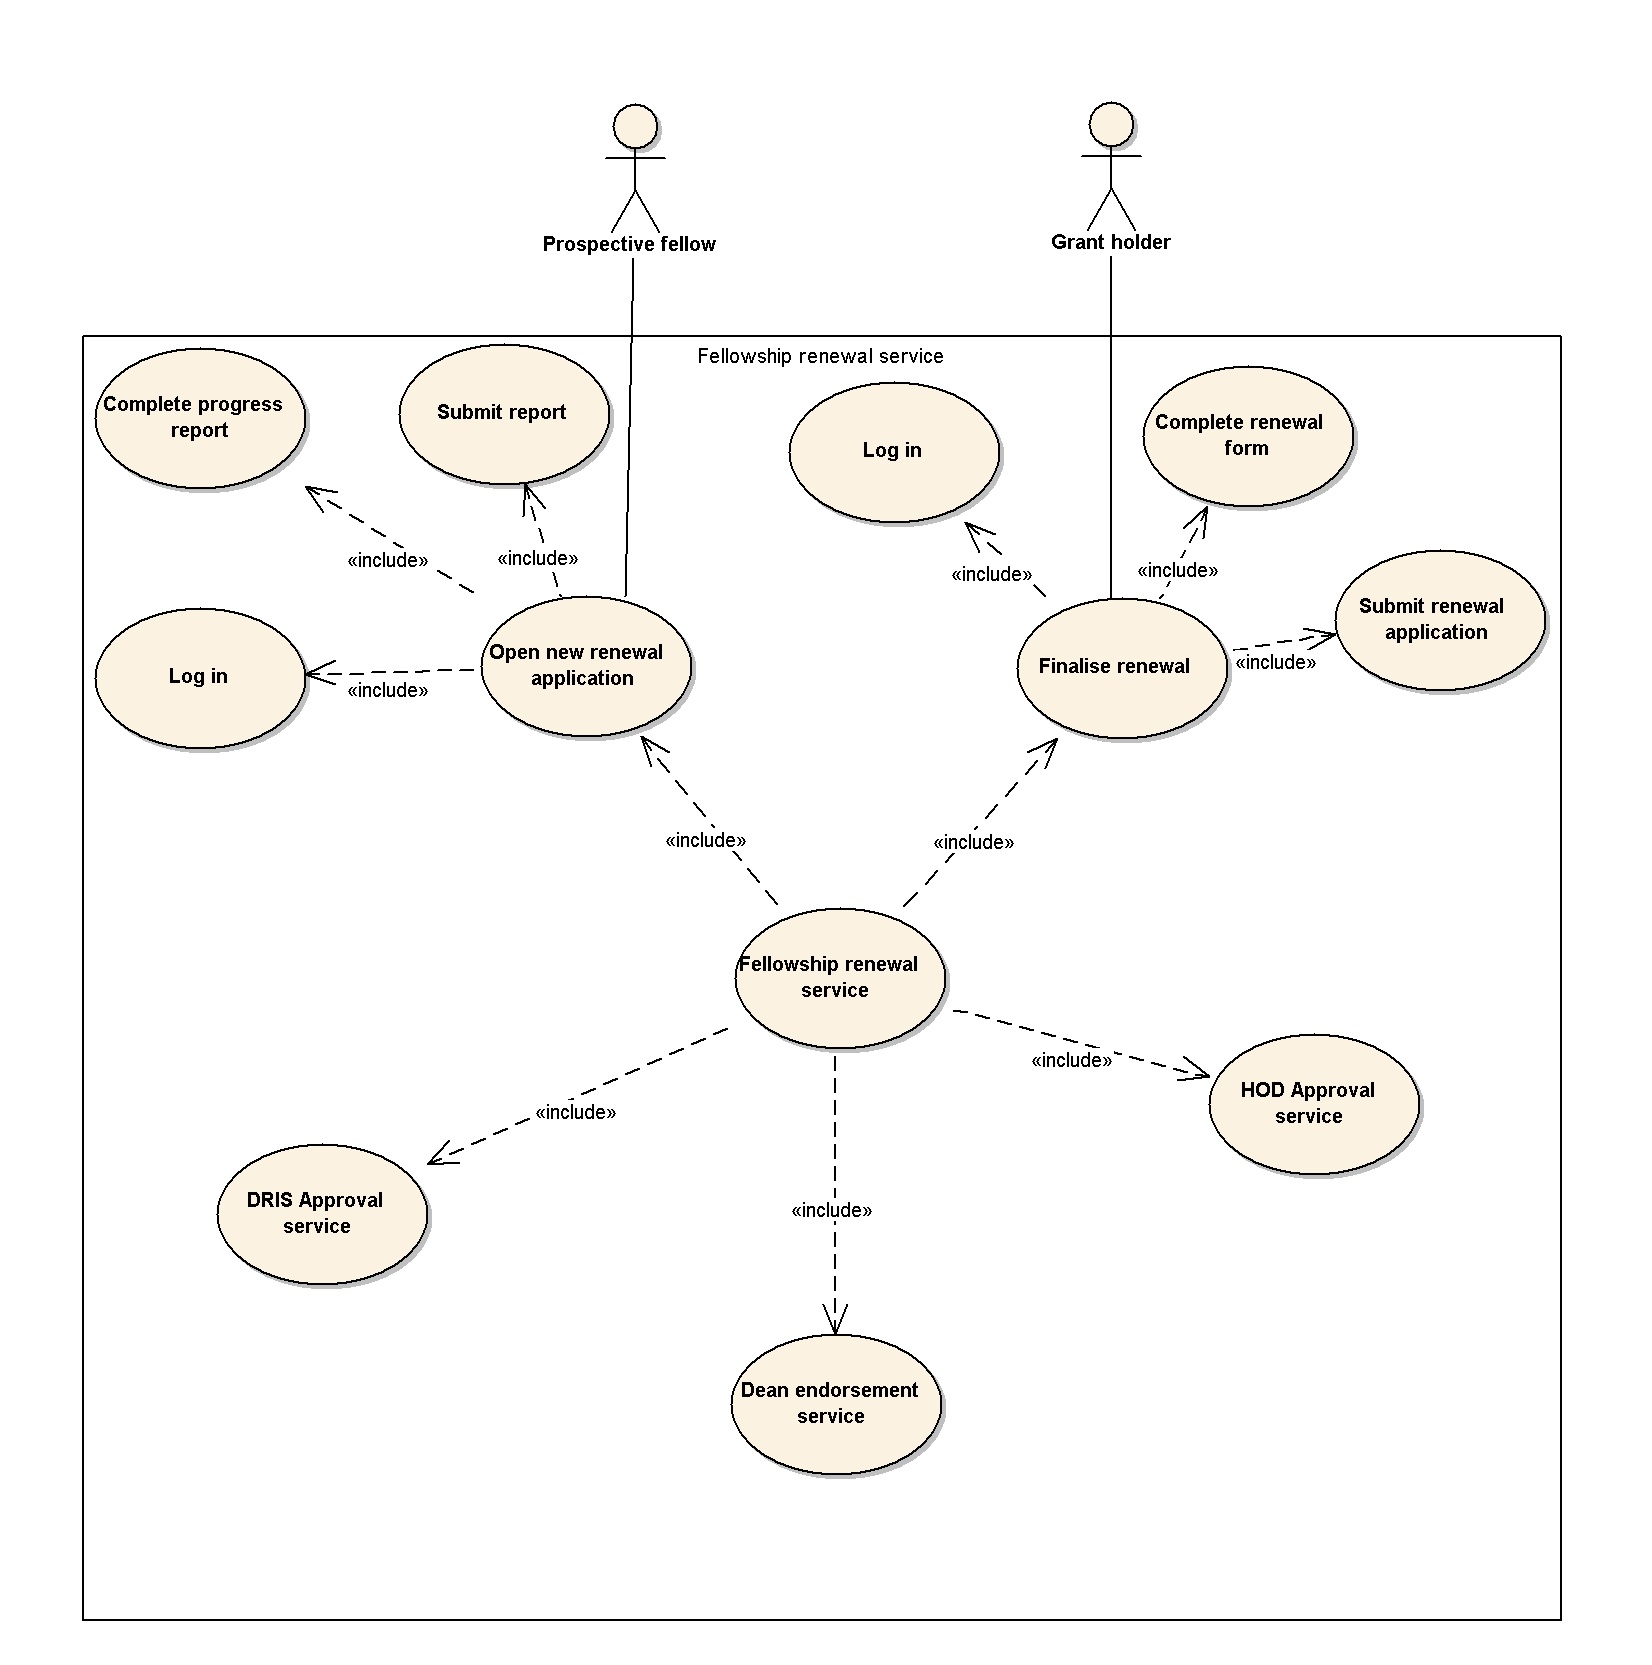
\includegraphics[scale=0.6]{./Pictures/Diagrams/Application/Fellowship renewal service.jpg}}
\caption{Use case diagram of Fellowship renewal service}
\end{figure}

\begin{figure}[H]
\centering	
\framebox{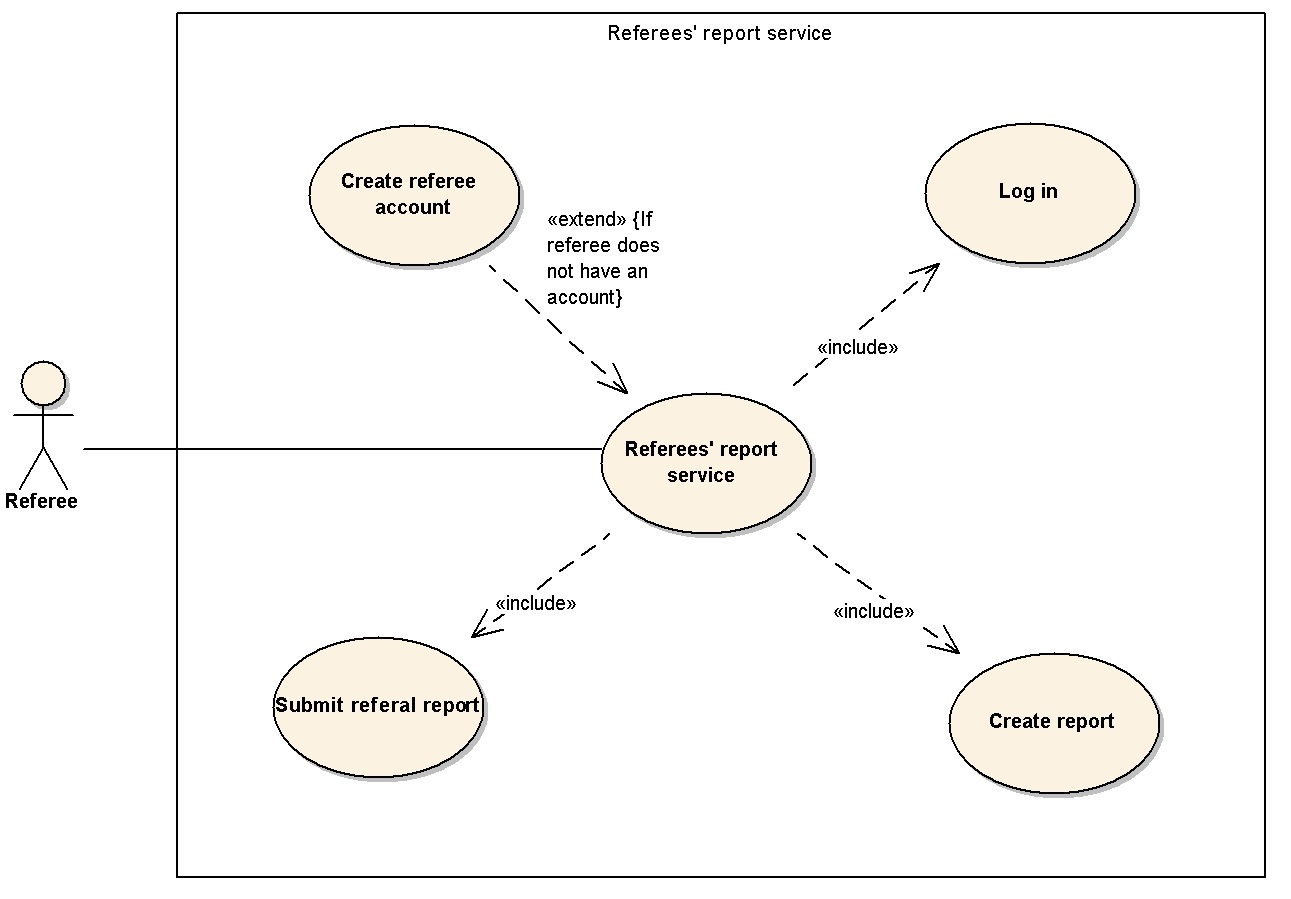
\includegraphics[scale=0.6]{./Pictures/Diagrams/Application/Referees' report service.jpg}}
\caption{Use case diagram of Referees' report service}
\end{figure}

\begin{figure}[H]
\centering	
\framebox{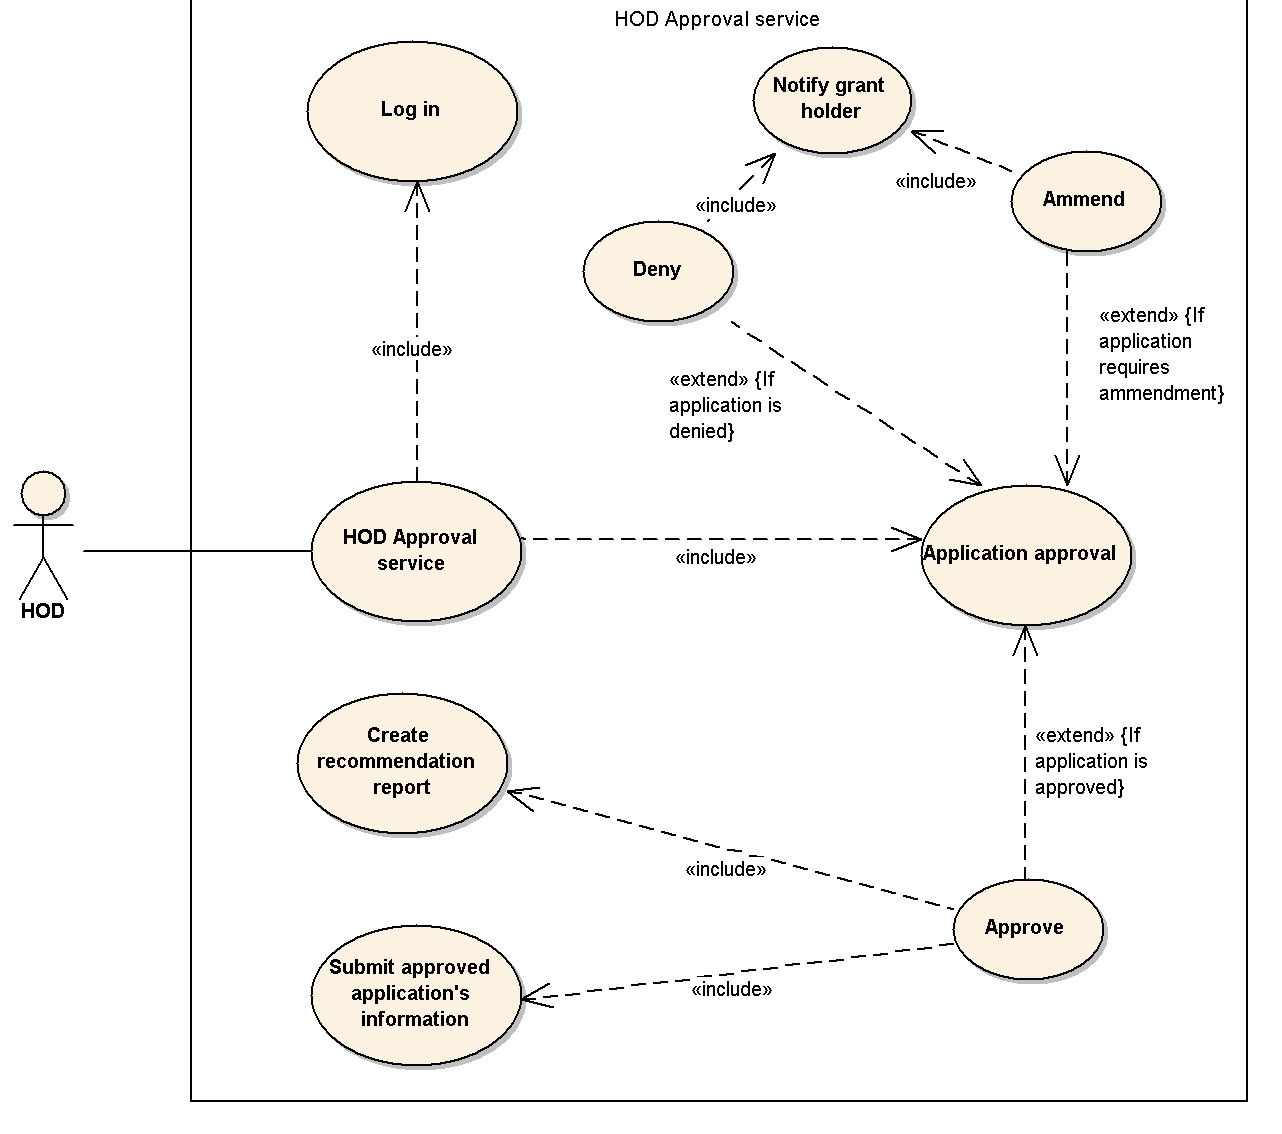
\includegraphics[scale=0.6]{./Pictures/Diagrams/Application/HOD Approval service.jpg}}
\caption{Use case diagram of HOD Approval service}
\end{figure}

\begin{figure}[H]
\centering	
\framebox{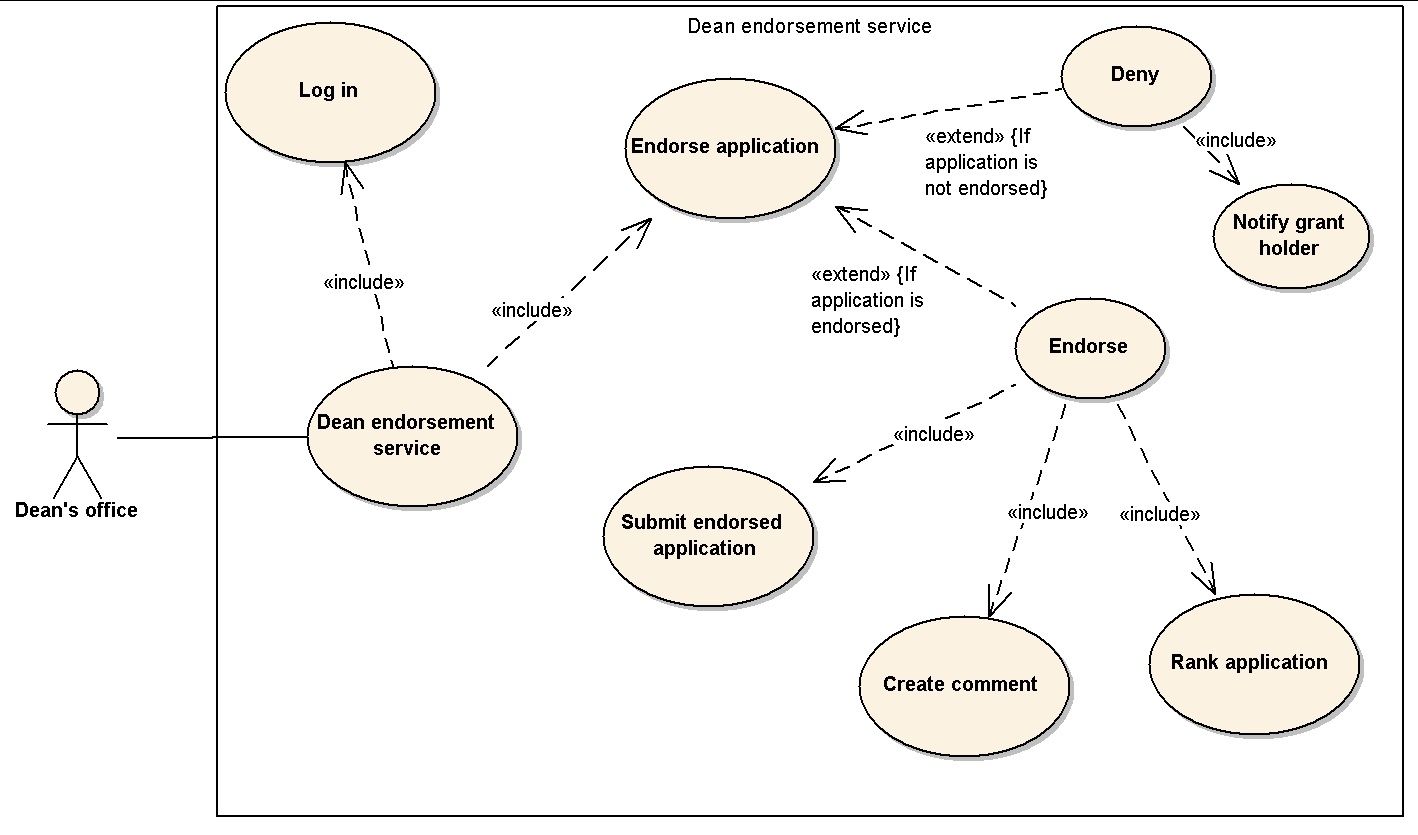
\includegraphics[scale=0.6]{./Pictures/Diagrams/Application/Dean endorsement service.jpg}}
\caption{Use case diagram of Dean endorsement service}
\end{figure}

\begin{figure}[H]
\centering	
\framebox{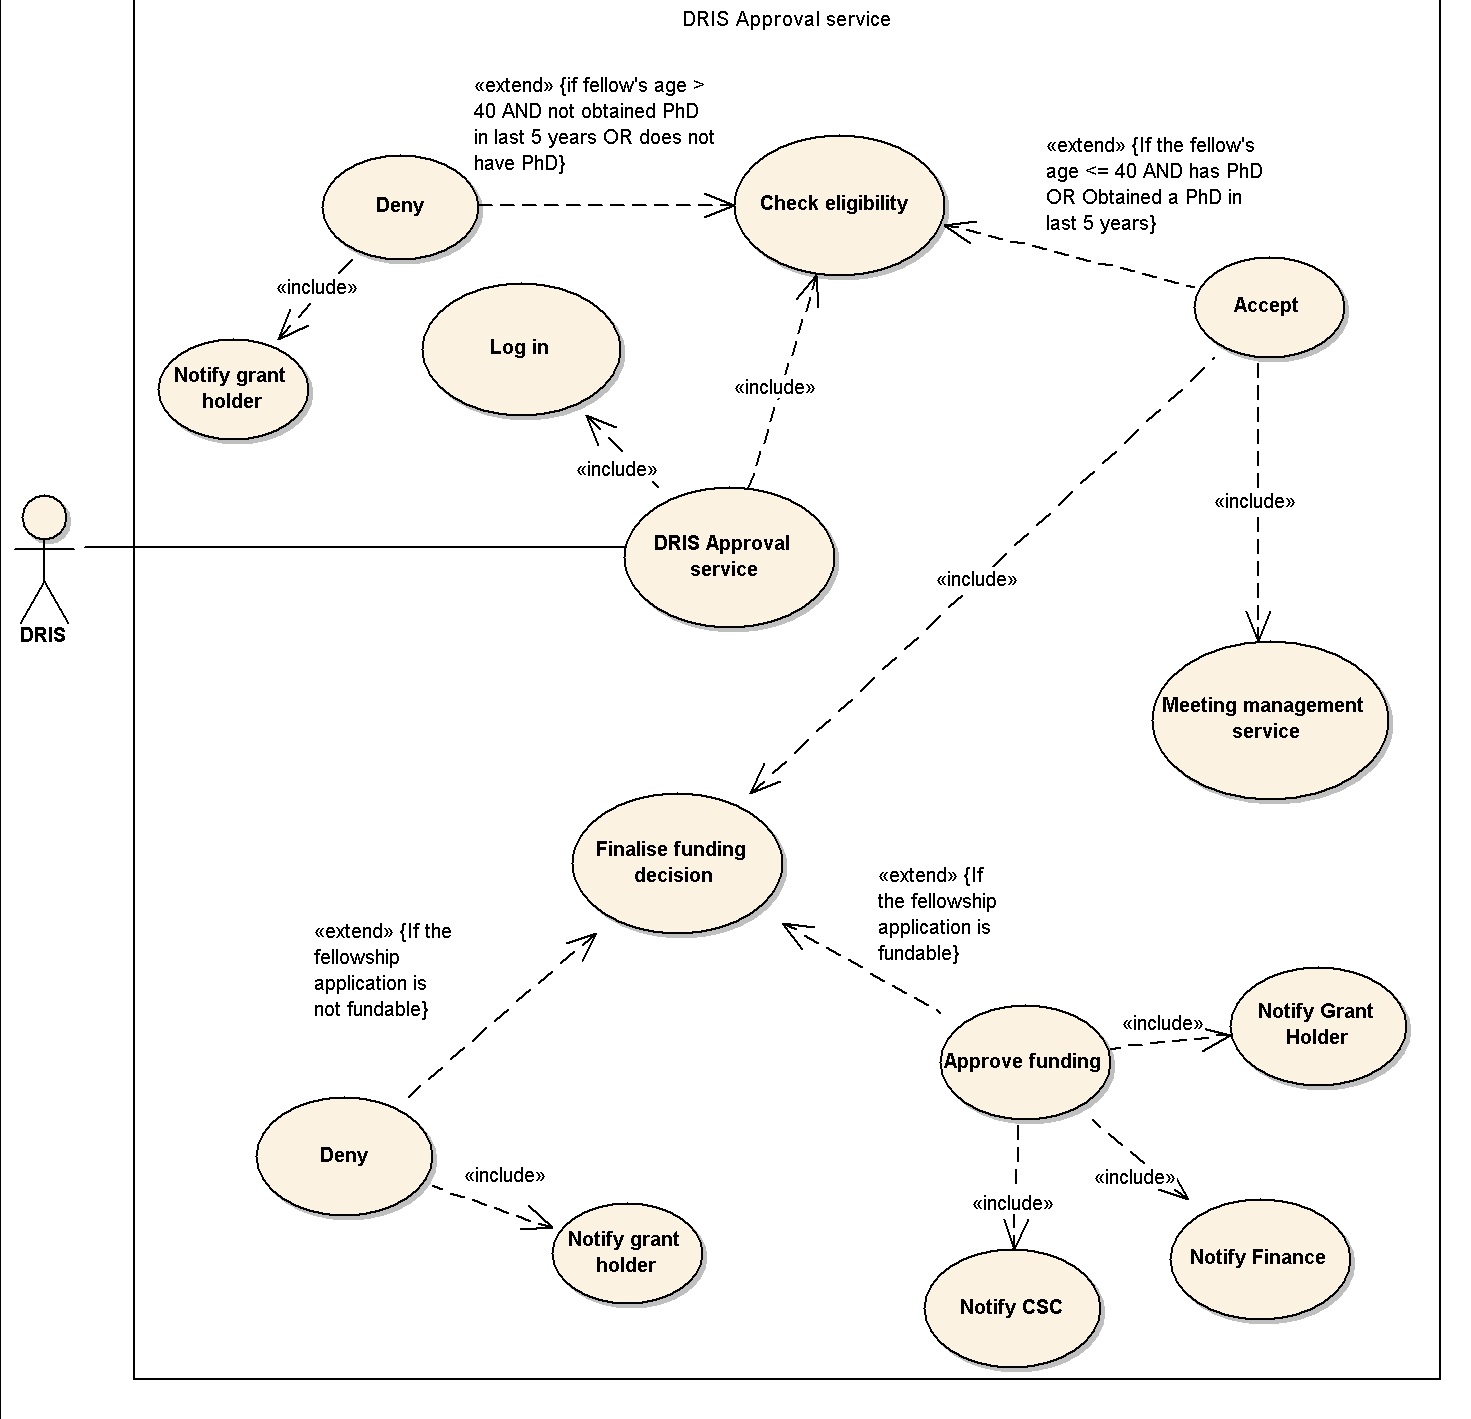
\includegraphics[scale=0.6]{./Pictures/Diagrams/Application/DRIS approval service.jpg}}
\caption{Use case diagram of DRIS approval service}
\end{figure}

\begin{figure}[H]
\centering	
\framebox{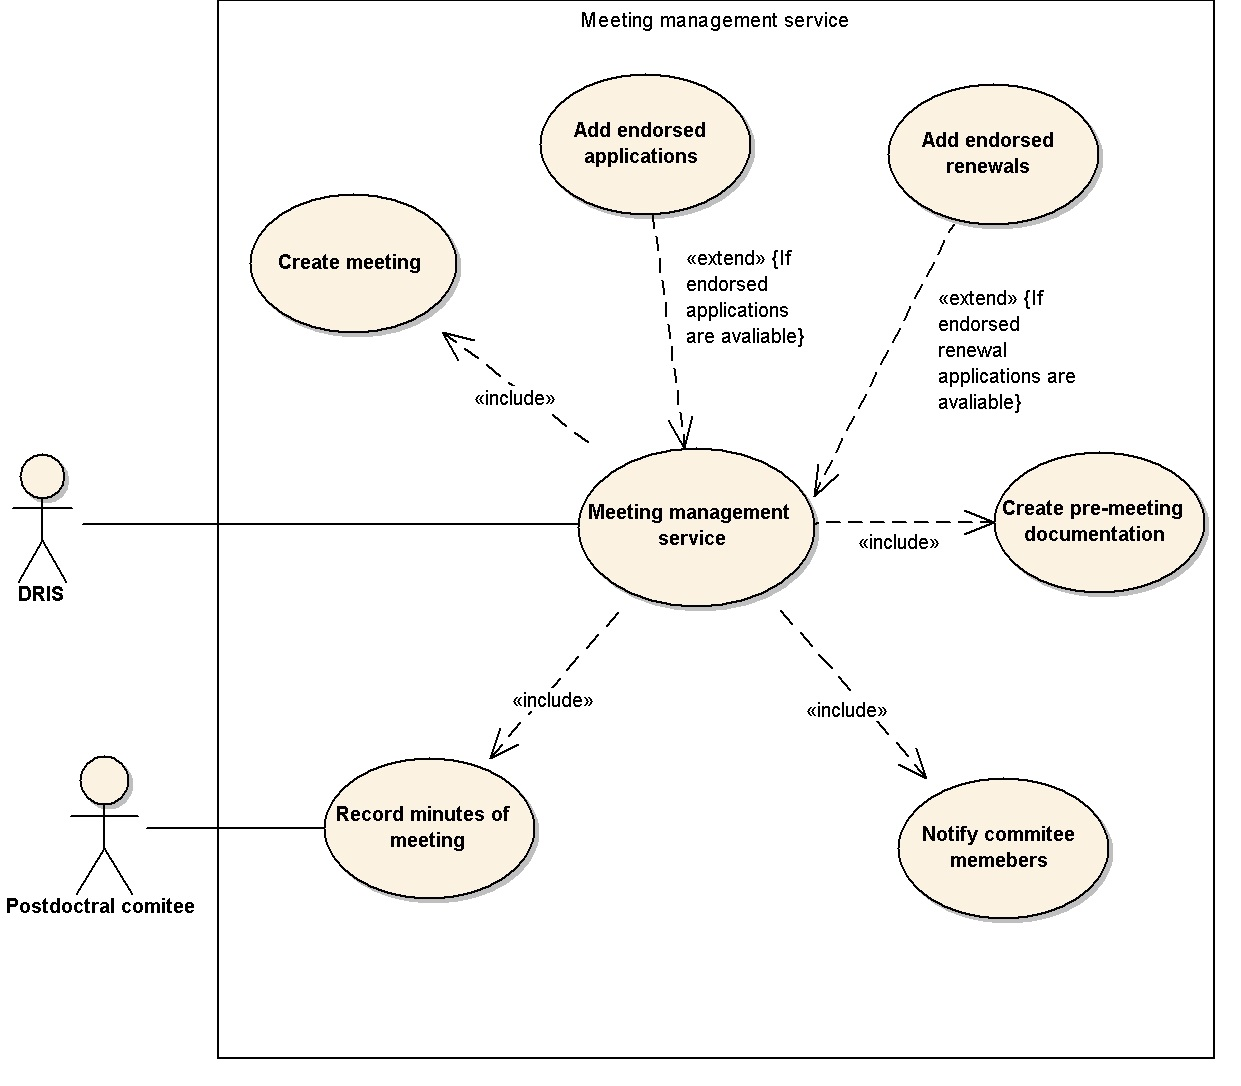
\includegraphics[scale=0.6]{./Pictures/Diagrams/Application/Meeting management service.jpg}}
\caption{Use case diagram of Meeting management service}
\end{figure}

\vspace{0.2in}
\subsubsection{Exclusions}
\vspace{0.2in}
Everything not included in this document in terms of scope is considered not in the scope of the project.
\vspace{0.2in}

\subsection{Required functionality} %Alfred
\vspace{0.2in}
The following sections will discuss the required functionality of all the major services handled by the system. Namely:
\begin{itemize}
\item Application service
\item Report services
\item Notification services
\item User account management services
\end{itemize}

%Use the use case diagrams to complete the requirements of each of the services in the format I provided
\subsubsection{Application services}
		Th main user of these services will be the prospective fellows who wishes to track their application progress or renew or apply for a Post-Doctoral fellowship. Other stakeholders will only make use of certain sub-services which are provided under the Application services:
		
		\begin{itemize}
			\item New fellowship application service API:		
			\begin{enumerate}
				\item Account creation for new prospective fellows, referees and grant holders.
				\item All internal stakeholders should be able to log in with their PeopleSoft account details.				
				\item A prospective fellow should be able to open a new application. 
				\item A prospective fellow should be able to add their CV in the required format. 
				\item A specified grant holder should be able to add their CV in the required format.
				\item A prospective fellow should be able to specify their intended grant holder.	
				\item A prospective fellow should be able to specify their intended referees.
				\item A specified grant holder should be able to complete prospective fellows application.
				\item A application should be made available for stakeholders such as the DRIS, HOD and Dean to endorse and approve it.		
			\end{enumerate}
			
			\item Fellowship renewal service API:
			\begin{enumerate}		
				\item All internal stakeholders should be able to log in with their PeopleSoft account details.	
				\item A fellow should be able to open a new renewal application. 
				\item A fellow should be able to add their progress report on all the work they have been working on. 
				\item A fellows' grant holder should be able to finalise the renewal application.
				\item The renewal application should be made available to the DRIS, HOD and dean for endorsement and approval.				
			\end{enumerate}
			\item Application progress viewer service API:
			\begin{enumerate}
				\item A prospective fellow should be able to login with their user specified account details.
				\item A prospective fellows application status should be made available for their consideration.			
			\end{enumerate}
		\end{itemize}

Once the steps are completed the applicants application is now under consideration. The applicant will also be able to see the status of the the applications current state through the whole application process.
\subsubsection{Report services}
The report use cases provides the uses for report generation such as the generation of an applications current status, or for use required by the DRIS.
\begin{enumerate}
	\item DRIS stakeholder must be logged into the system.
	\item The DRIS must be able to create a report which effectively allows them to:
	\begin{itemize}
		\item Open new report.
		\item Select report data.
		\item Generate report.
		\item View report.
	\end{itemize}
	\item The viewing of a report must allow the report to be exported to either a pdf or a spreadsheet.
\end{enumerate}
\subsubsection{User account management services} %Couldn't see who the actor is on the use case diagram
\begin{itemize}
	\item Allow users to login.
	\item The service must be able to create new account.
	\item Modify account details.
	\item Remove and account.
\end{itemize}
\subsubsection{Notification services}
Every participant is due to receive notifications regarding their actions every now and then. This service is to follow these steps:
\begin{itemize}
	\item Stakeholders must be able to create a new notification.
	\item Notification must have recipient.
	\item Notification must have a non-empty message.
	\item Notification can  be sent as email or to a user account.
\end{itemize}
\vspace{0.2in}
\subsection{Use case prioritization} %Alfred
\vspace{0.2in}
This section states the ranking in terms of priority of the each use case per use case diagram figure. The priorities are: Critical, Important and Nice to have.\\ 
\begin{itemize}
	\item Application services: Critical
	\begin{itemize}
		\item New Application: Critical
		\item Renewal Application: Critical
		\item Application progress viewer service: Important
		\item Meeting management service: Nice To Have
	\end{itemize}
	\item Report services: Important
	\item Notification services: Critical
	\item User account management services: Critical
	\begin{itemize}
		\item Create new account: Critical
		\item Modify account: Critical
		\item Remove account: Critical
		\item Login: Ciritical
	\end{itemize}
	\item 
\end{itemize}


\vspace{0.2in}

\subsection{Use case/Services contracts} %Mathys
\vspace{0.2in}

This section states the preconditions and postconditions of the each use case per use case diagram figure. \\

\subsubsection{Preconditions}
These are conditions that must be met by the system or user before they are allowed to use the use case.\\
\begin{itemize}
	\item Fig 2.
	\begin{itemize}
		\item New fellowship application service: Can only be accessed if new applications are open.
		\item Fellowship renewal service: Can only be accessed if renewals are open.
		\item Application progress viewer service: Can only be accessed if user logged in with correct security permissions.	
	\end{itemize}
	
	\item Fig 3.
		\begin{itemize}
			\item Log in: If a user with the associated credentials has appropriate security role.
			\item Create report: If user is logged in.
			\item Open new report: If no report is currently open.
			\item Select report data: If report is open and data is available for report.
			\item Generate report: If data has been selected.
			\item View report: If a report has been generated.
			\item Export report: If user wants to export report.
			\item To spreadsheet: If user wants to export report to a spreadsheet.
			\item To pdf: If user wants to export report to a pdf.	
		\end{itemize}
	
	\item Fig 4.
			\begin{itemize}
				\item Create notification: If requesting user is the system.
				\item Specify recipient user account: If a notification is in its setup stage.				
				\item Specify message: If a notification is in its setup stage.
				\item Send user account notification: If notification is ready to be sent.
				\item Send email: If notification is ready to be sent.	
			\end{itemize}
	
	\item Fig 5.
			\begin{itemize}
				\item Create new account: If requesting user has the appropriate security role.
				\item Modify account: If requesting user has the appropriate security role or is the owner of the account.				
				\item Remove account: If requesting user has the appropriate security role.						
			\end{itemize}
	
	\item Fig 6.
		\begin{itemize}
			\item View application progress: Can only be used if there are any applications made by the user.
		\end{itemize}
		
	\item Fig 7.
		\begin{itemize}
			\item Create prospective fellow account: If prospective fellow does not have an account.
			\item Submit information: If all the application information is complete.				
			\item Create grant holder account: If grant holder does not have an account.
			\item Create grant holder cv: If the grant holder does not have an NRF rating or does have never created a CV on the system before.
			\item Submit application: If all the required information has been entered.									
		\end{itemize}
	
	\item Fig 8.
		\begin{itemize}
			\item Open new renewal application: If prospective fellow has a fellowship that is renewable.
			\item Submit report: If progress report is completed.				
			\item Submit renewal application: If all the required information for the renewal has been entered.									
		\end{itemize}
	
	\item Fig 9.
		\begin{itemize}
			\item Create referee account: If the referee does not have an account.
			\item Create report: If requesting user has the appropriate security role.				
			\item Submit referral report: If the referral report has been completed.									
		\end{itemize}
		
	\item Fig 10.
		\begin{itemize}
			\item Application approval: If any finalised application is available for approval and the grant holder of the application falls under department the HOD is in charge of.
			\item Create recommendation report: If the application has been approved.				
			\item Submit approved application's information: If the recommendation report has been completed.									
		\end{itemize}
		
	\item Fig 11.
		\begin{itemize}
			\item Endorse application: If any approved application is available for endorsement and the grant holder of the application falls under faculty of which the Dean's office is in charge of.
			\item Rank application: If the application has been endorsed.	
			\item Create comment: If the application has been ranked.			
			\item Submit endorsed application: If the required endorsement information has been completed.									
		\end{itemize}
	
	\item Fig 12.
		\begin{itemize}
			\item Check eligibility: If any endorsed application is available for its eligibility check.
			\item Deny: If the prospective fellow is older than 40 and has not obtained their PhD in the last 5 years or if the prospective fellow does not have a PhD.
			\item Accept: If the prospective fellow is younger than 40 or is 40 and they have a PhD or if they have obtained a PhD in the last 5 years. 
			\item Finalise funding decision: If the meeting regarding the application has been concluded.	
			\item Deny: If the application's funding was denied.			
			\item Approve funding: If the application's funding was denied.									
		\end{itemize}
	
	\item Fig 13.
		\begin{itemize}
			\item Create meeting: If any eligible applications are available.
			\item Add endorsed applications: If any new applications that are eligible are available.
			\item Add endorsed renewals: If any renewal applications that are eligible are available.
			\item Record minutes of meeting: If the selected meeting has been setup.							
		\end{itemize}
	\end{itemize}

\subsubsection{Postconditions}
These are conditions that must be met by the system and the data after the use case has been used.\\
\begin{itemize}
		
	\item Fig 3.
		\begin{itemize}
			\item Log in: The user has been authenticated and has the appropriate security role.
			\item Open new report: A new report is active.
			\item Select report data: The data for the active report is selected.
			\item Generate report: The report is available for viewing.
			\item View report: The report is available for export and must be visible.	
		\end{itemize}
	
	\item Fig 4.
			\begin{itemize}
				\item Create notification: A possible notification is open for receiving its contents.
				\item Specify recipient user account: The notification has a a recipient.				
				\item Specify message: The notification has a message.
				\item Send user account notification: The message is sent to the user.
				\item Send email: The message is sent the email associated with recipients user account.	
			\end{itemize}
	
	\item Fig 5.
			\begin{itemize}
				\item Create new account: A new user account is added to the system.
				\item Modify account: The specified user account is updated.				
				\item Remove account: The specified user account is removed from the system.						
			\end{itemize}
	
	\item Fig 6.
		\begin{itemize}
			\item View application progress: The application progress of the specified user application is visible.
		\end{itemize}
		
	\item Fig 7.
		\begin{itemize}
			\item Create prospective fellow account: If prospective fellow has an account.
			\item Create prospective fellow cv: The CV is created and associated with the prospective fellow and the application.
			\item Specify grant holder: The grant holder's contact information is associated with the application.
			\item Specify referees: The referees' contact information is associated with the application.
			\item Submit information: The initial application data is complete. Referees are notified.				
			\item Create grant holder account: The grant holder has an account.
			\item Create grant holder cv: The grant holder's CV is associated with the application.
			\item Complete application form: The application data is complete and the application is ready to be finalised.
			\item Submit application: The application is now a finalised application and the HOD of the relative department is notified. 									
		\end{itemize}
	
	\item Fig 8.
		\begin{itemize}
			\item Open new renewal application: A new renewal is for a fellowship is open.
			\item Log in: The user has been authenticated and has the appropriate security role.
			\item Complete progress report: The progress report associated with	the renewal.		
			\item Submit report: The initial renewal information is complete. Grant holder is notified.
			\item Complete renewal form: The renewal data complete and the renewal is ready to be finalised.			
			\item Submit renewal application: The renewal application is finalised and the HOD of the relative department is notified.									
		\end{itemize}
	
	\item Fig 9.
		\begin{itemize}
			\item Create referee account: Referee has a user account.
			\item Log in: The user has been authenticated and has the appropriate security role.
			\item Create report: The report is complete and ready to be submitted.				
			\item Submit referral report: The referral report has been finalised and associated with the application and the Grant Holder of the application is notified.									
		\end{itemize}
		
	\item Fig 10.
		\begin{itemize}
			\item Log in: The user has been authenticated and has the appropriate security role.
			\item Deny: Application has status changed to denied.
			\item Amend: Application is reopened and status changed to amend.
			\item Notify grant holder: A notification is sent to the Grant holder of the application.  
			\item Approve:  The application recommendation report becomes available for completion.
			\item Create recommendation report: The recommendation report is associated with the application and the Approval is ready to be finalised.				
			\item Submit approved application's information: The application approval is finalised and the application is now a approved application and the Dean's Office of the relevant faculty is notified.									
		\end{itemize}
		
	\item Fig 11.
		\begin{itemize}
			\item Log in: The user has been authenticated and has the appropriate security role.
			\item Deny: The application's status is changed to denied. 
			\item Notify grant holder: A notification is sent to the Grant holder of the application.
			\item Endorse: The application's endorsement information becomes available for completion.
			\item Rank application: The application has a rank associated with it.	
			\item Create comment: The application has a endorsement comment associated with it.			
			\item Submit endorsed application: The application endorsement is finalised and the application is now an endorsed application and the DRIS is notified.									
		\end{itemize}
	
	\item Fig 12.
		\begin{itemize}
			\item Log in: The user has been authenticated and has the appropriate security role.
			\item Deny: The application's status is changed to denied. 
			\item Notify grant holder: A notification is sent to the Grant holder of the application.
			\item Accept: The application is ready for discussion and is now an eligible application.			
			\item Deny: The application's status is changed to denied.			
			\item Approve funding: The application is now a complete application.
			\item Notify grant holder: A notification is sent to the Grant holder of the application.
			\item Notify CSC: A notification is sent to the CSC.
			\item Notify Finance: A notification is sent to the Finance department.									
		\end{itemize}
	
	\item Fig 13.
		\begin{itemize}
			\item Create meeting: A new meeting is open for modification.
			\item Add endorsed applications: An endorsed new application has been added to the agenda of the meeting.
			\item Add endorsed renewals: An renewal application has been added to the agenda of the meeting.
			\item Create pre-meeting documentation: Documentation complete and associated with meeting and the meeting is closed for modification.
			\item Notify committee members: A notification is sent to all the committee members.
			\item Record minutes of meeting: The meeting is finalised and it's minutes stored.							
		\end{itemize}

\end{itemize}


\vspace{0.2in}

%\subsection{Process specifications} %Alfred
%\vspace{0.2in}

%\vspace{0.2in}

\subsection{Domain Objects} %Alfred
\subsubsection{Overview}

\begin{figure}[H]
\centering	
\framebox{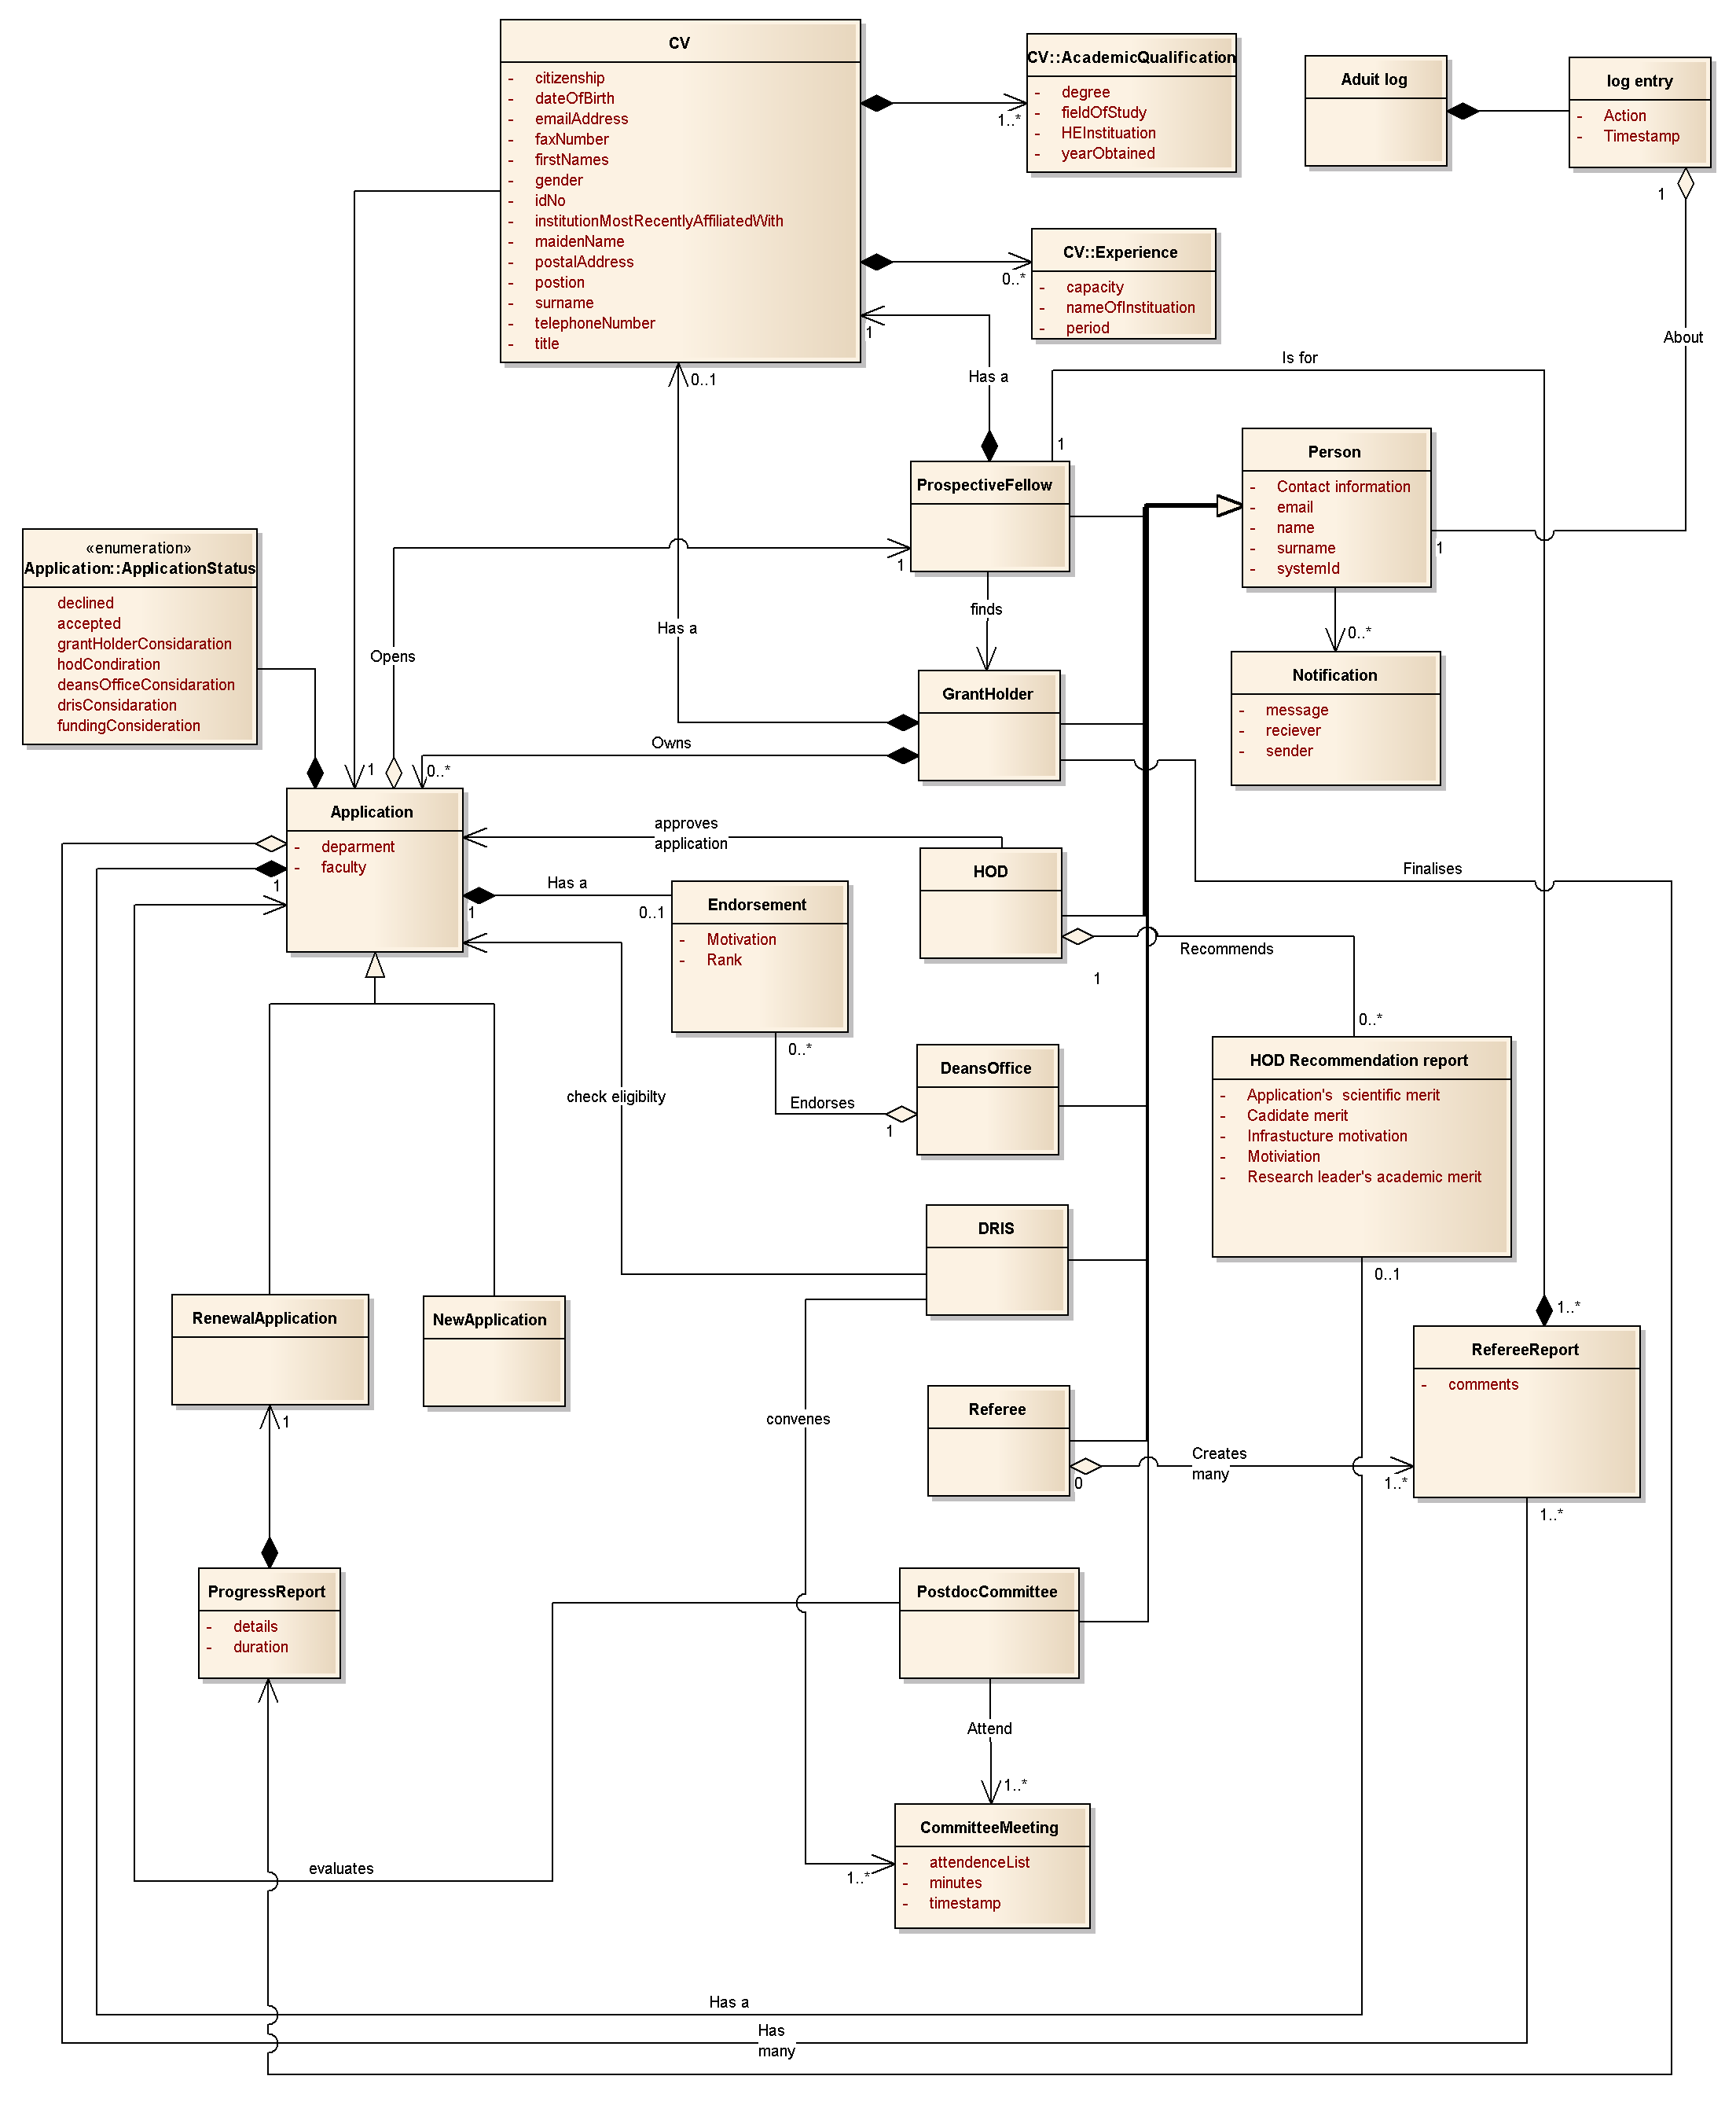
\includegraphics[scale=0.55]{./Pictures/Diagrams/DomainObjects/DomainObjects.png}}
\caption{Overview of the data structures and relationships for the core domain objects of the
system.}
\end{figure}

\newpage
\subsubsection{Persons}
This object represents the stakeholders that will make use of the system. All stakeholders will have accounts which they use to log on to the system with a unique user id and a predefined or user specified password. The unique user id can ethier be a Peoplesoft Emplid number or a email address.

\subsubsection{DRIS}
The Department of Research and Innovation Support who administers the process.

\subsubsection{ProspectiveFellow}
Required to be a holder of a PhD obtained in the last five years (or nearing completion of a PhD) or is 40 years or younger and has a PhD.

\subsubsection{Grant holder}
Grant holders are possibly rated researchers by the NRF and the system should not require the CV's of A and B rated researchers to be added to the system. The reason for this is that the CV's of such researchers are very long. Will be the supervisor for the fellow and submits the application.

\subsubsection{HOD}
Has to indicate whether the department  is able to host the prospective fellow and is satisfied with the quality of the fellow, and that the aims are aligned with the University’s strategic plans.\\

Approves new and renewal applications (including referee reports) and submits to Dean or Deputy Dean of Research

\subsubsection{Deans Office}
Dean's office of the relevant faculty/ Deputy Dean of Research who approves the application for the faculty.

\subsubsection{Referee}
Will provide referee report regarding the student.

\subsubsection{PostDocComittee}
The commitee who approves applicaitons during committee meetings.

\subsubsection{Application}
Applications will contain the required info of a prospective fellow, e.g. CV and academic record, and who their researcher leader (grant holder) is. The status of the application will be accessible in reports for all stakeholders. The status will either be draft, pending (under consideration), denied or accepted. The status will contain details regarding to why it is in the current state.

\subsubsection{NewApplication}
Application from a prospective fellow who is currently not a fellow in the system.

\subsubsection{RenewalApplication}
Renewal application from a prospective fellow already in the system.

\subsubsection{ProgressReport}
Report on the work that the fellow had done through the duration of their fellowship.

\subsubsection{CV}
Contains information (personal details, academic experience and work experience) regarding a person (grant holder or prospective fellow) in the system.

\subsubsection{HODRecommandationReport}
Report highlighting reasons to why prospective fellow is needed by the department.

\subsubsection{Notification}
Used as a means for persons to communicate within (or possible out of)  the system

\subsubsection{LogEntry}
Used for audit trail for acions committed by persons in the system.

\subsubsection{AuditLog}
Audits actions by users within the system.

\subsubsection{Endorsement}
Endorsement of an application once it has been approved and ranked by the dean..

\subsubsection{Post-doctoral committee meetings}
The post-doctoral committee will be assessing the applications and will evaluate and give an application a ranking.

\newpage	
\section{Open Issues:} %Everyone
\vspace{0.2in}

\begin{itemize}
\item Theft or loss of mobile devices
\item User errors like typing errors
\item How will an applicant be allocated a student number?
\item Should the system treat a prospective fellow in a unique class or a should all stakeholders be of the same class and be allocated different roles, as someone could work as a stakeholder but still want to apply?
\item Automating a check for the rating of researchers.
\item The CVs of A and B rated researchers was not added to save paper. Should we still not add it to keep it more convenient for the researchers?
\end{itemize}


\vspace{0.5in}

\newpage
\section{Glossary:} %Mathys
\vspace{0.2in}

\begin{itemize}


\item \textbf{CV} - Curriculum Vita
\item \textbf{PDF} - Portable Document Format file
\item \textbf{NRF} - National Research Foundation
\item \textbf{API} - Application Programming Interface
\item \textbf{Spreadsheet} - A special type of computer document that is used to represent data in rows and columns. 
\item \textbf{HTML} - Hyper Text Mark-up Language
\item \textbf{Java EE} - Java Enterprise Edition
\item \textbf{Use case} - A visual depiction of a service or group of services.
\item \textbf{Application} - Both a renewal and new fellowship are seen as applications.
\item \textbf{PhD} - A doctoral degree in a particular field of study. 


\end{itemize}	


\vspace{0.5in}


\end{document}